\begin{enumerate}[label=\thesection.\arabic*.,ref=\thesection.\theenumi]
\numberwithin{equation}{enumi}
\item An op amp designed to have a low-frequency gain of $10^{5}$ and a high-frequency response dominated by a single pole at 100 rad/s, acquires, through a manufacturing error, a pair of additional poles at 10,000 rad/s. 
\begin{enumerate}
\item At what frequency does the total phase shift reach 180$\degree$ ? 
\item At this frequency, for what value of H, assumed to be frequency independent, does the loop gain reach a value of unity? 
\item What is the corresponding value of closed-loop gain at low frequencies?
\end{enumerate}
\solution
\begin{align}
G(s) &= \frac{G_{0}}{1+\frac{s}{p}} 
\end{align}
Considering manufacturing error
\begin{align}
G(s) &= \dfrac{G_{0}}{\brak{1+\dfrac{s}{p}}\brak{1+\dfrac{s}{p_{error}}}} 
\\
G_{0} &= \text{Low Frequency Gain} = 10^{5}
\\
p &= 100
\\
p_{error} &= 10^{4}
\\
G(s) &= \dfrac{10^{5}}{\brak{1+\dfrac{s}{100}}\brak{1+\dfrac{s}{10^{4}}}^{2}}
\\
\measuredangle G(j\omega) &= -\tan^{-1}\frac{\omega}{100} - 2\tan^{-1}\frac{\omega}{10^{4}}
\end{align}
\item Calculating the frequency at which the total phase shift reach 180$\degree$ 

At $\omega_{180}, \measuredangle G(j\omega_{180}) = -180\degree$

Also $\omega_{180} >> 100$
\begin{align}
180\degree &= 90\degree  + 2 \tan^{-1}\brak{\frac{\omega_{180}}{10^{4}}}
\\
\tan^{-1}\frac{\omega_{180}}{10^{4}}&= 45\degree
\\
\frac{\omega_{180}}{10^{4}} &= \tan 45\degree = 1
\\
\omega_{180} &= 10^{4} rad/s
\end{align}
\begin{figure}[!ht]
\centering
    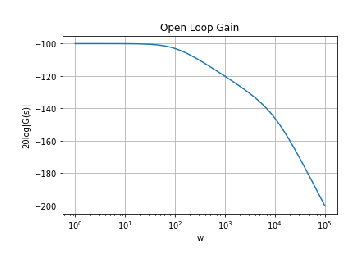
\includegraphics[width=\columnwidth]{./figs/Figure_1.eps}
  \caption{Open Loop Gain}
  \label{fig:plot1}
\end{figure}
\item Calculating feedback factor $H$ for which loop gain at $\omega_{180}$ is unity
\begin{align}
\text{Loop Gain} = G(s)H = 1
\\
\dfrac{10^{5}H}{\sqrt{1^{2} + \brak{\dfrac{\omega_{180}}{10^{2}}}^{2}} \sqrt{\brak{1+\dfrac{\omega_{180}}{10^{4}}}^{2}}} = 1
\\
H = 0.002
\end{align}
\item Calculating the closed loop gain at low frequency
Let $T(s)$ be the closed loop Transfer Function.
\begin{figure}[!hbt]
	\begin{center}
			\resizebox{\columnwidth}{!}{\tikzstyle{block} = [draw, fill=blue!20, rectangle, 
    minimum height=3em, minimum width=4em]
\tikzstyle{sum} = [draw, fill=blue!20, circle, node distance=1cm]
\tikzstyle{input} = [coordinate]
\tikzstyle{output} = [coordinate]
\tikzstyle{pinstyle} = [pin edge={to-,thin,black}]

\begin{tikzpicture}[auto, node distance=2cm]
    \node [input, name=input] {$V_s$};
    \node [sum, right of=input] (sum) {};
    \node [block, right of=sum] (controller) {$G(s)$};
    \node [output, right of=controller] (output) {};
    \node [block, below of=controller] (feedback) {$H$};
    \draw [draw,->] (input) -- node {$V_s$} (sum);
    \draw [->] (sum) -- node {$V_i$} (controller);
    \draw [->] (controller) -- node [name=y] {$V_o$}(output);
    \draw [->] (y) |- (feedback);
    \draw [->] (feedback) -| node[pos=0.99]{$-$}  node [near end] {$V_f$} (sum);
\end{tikzpicture}}
	\end{center}
\caption{Closed loop circuit}
\label{fig:equivalent_system}
\end{figure}

\begin{align}
T(s) &= \dfrac{G(s)}{1+H G(s)}
\\
T(s) &= \dfrac{10^{5}}{H 10^{5}+ \brak{1+\dfrac{s}{100}}\brak{1+\dfrac{s}{1000}}^{2}}
\\
T(s) &= \dfrac{10^{5}}{10^{-10} s^{3} + (2x10^{-6}) s^{2} + 10^{-2}s + 1 + 10^{5}H}
\end{align}
At low frequencies
\begin{align}
T(0) &= \dfrac{10^{5}}{1 + 10^{5}H}
\\
|T(0)| &= \dfrac{10^{5}}{\sqrt{(200)^{2}}}
\end{align}

\begin{align}
|T(0)| &= 500 V/V
\end{align}

\begin{table}[!ht]
\centering

%%%%%%%%%%%%%%%%%%%%%%%%%%%%%%%%%%%%%%%%%%%%%%%%%%%%%%%%%%%%%%%%%%%%%%
%%                                                                  %%
%%  This is the header of a LaTeX2e file exported from Gnumeric.    %%
%%                                                                  %%
%%  This file can be compiled as it stands or included in another   %%
%%  LaTeX document. The table is based on the longtable package so  %%
%%  the longtable options (headers, footers...) can be set in the   %%
%%  preamble section below (see PRAMBLE).                           %%
%%                                                                  %%
%%  To include the file in another, the following two lines must be %%
%%  in the including file:                                          %%
%%        \def\inputGnumericTable{}                                 %%
%%  at the beginning of the file and:                               %%
%%        \input{name-of-this-file.tex}                             %%
%%  where the table is to be placed. Note also that the including   %%
%%  file must use the following packages for the table to be        %%
%%  rendered correctly:                                             %%
%%    \usepackage[latin1]{inputenc}                                 %%
%%    \usepackage{color}                                            %%
%%    \usepackage{array}                                            %%
%%    \usepackage{longtable}                                        %%
%%    \usepackage{calc}                                             %%
%%    \usepackage{multirow}                                         %%
%%    \usepackage{hhline}                                           %%
%%    \usepackage{ifthen}                                           %%
%%  optionally (for landscape tables embedded in another document): %%
%%    \usepackage{lscape}                                           %%
%%                                                                  %%
%%%%%%%%%%%%%%%%%%%%%%%%%%%%%%%%%%%%%%%%%%%%%%%%%%%%%%%%%%%%%%%%%%%%%%



%%  This section checks if we are begin input into another file or  %%
%%  the file will be compiled alone. First use a macro taken from   %%
%%  the TeXbook ex 7.7 (suggestion of Han-Wen Nienhuys).            %%
\def\ifundefined#1{\expandafter\ifx\csname#1\endcsname\relax}


%%  Check for the \def token for inputed files. If it is not        %%
%%  defined, the file will be processed as a standalone and the     %%
%%  preamble will be used.                                          %%
\ifundefined{inputGnumericTable}

%%  We must be able to close or not the document at the end.        %%
	\def\gnumericTableEnd{\end{document}}


%%%%%%%%%%%%%%%%%%%%%%%%%%%%%%%%%%%%%%%%%%%%%%%%%%%%%%%%%%%%%%%%%%%%%%
%%                                                                  %%
%%  This is the PREAMBLE. Change these values to get the right      %%
%%  paper size and other niceties.                                  %%
%%                                                                  %%
%%%%%%%%%%%%%%%%%%%%%%%%%%%%%%%%%%%%%%%%%%%%%%%%%%%%%%%%%%%%%%%%%%%%%%

	\documentclass[12pt%
			  %,landscape%
                    ]{report}
       \usepackage[latin1]{inputenc}
       \usepackage{fullpage}
       \usepackage{color}
       \usepackage{array}
       \usepackage{longtable}
       \usepackage{calc}
       \usepackage{multirow}
       \usepackage{hhline}
       \usepackage{ifthen}



%%  End of the preamble for the standalone. The next section is for %%
%%  documents which are included into other LaTeX2e files.          %%
\else

%%  We are not a stand alone document. For a regular table, we will %%
%%  have no preamble and only define the closing to mean nothing.   %%
    \def\gnumericTableEnd{}

%%  If we want landscape mode in an embedded document, comment out  %%
%%  the line above and uncomment the two below. The table will      %%
%%  begin on a new page and run in landscape mode.                  %%
%       \def\gnumericTableEnd{\end{landscape}}
%       \begin{landscape}


%%  End of the else clause for this file being \input.              %%
\fi

%%%%%%%%%%%%%%%%%%%%%%%%%%%%%%%%%%%%%%%%%%%%%%%%%%%%%%%%%%%%%%%%%%%%%%
%%                                                                  %%
%%  The rest is the gnumeric table, except for the closing          %%
%%  statement. Changes below will alter the table's appearance.     %%
%%                                                                  %%
%%%%%%%%%%%%%%%%%%%%%%%%%%%%%%%%%%%%%%%%%%%%%%%%%%%%%%%%%%%%%%%%%%%%%%

\providecommand{\gnumericmathit}[1]{#1} 
%%  Uncomment the next line if you would like your numbers to be in %%
%%  italics if they are italizised in the gnumeric table.           %%
%\renewcommand{\gnumericmathit}[1]{\mathit{#1}}
\providecommand{\gnumericPB}[1]%
{\let\gnumericTemp=\\#1\let\\=\gnumericTemp\hspace{0pt}}
 \ifundefined{gnumericTableWidthDefined}
        \newlength{\gnumericTableWidth}
        \newlength{\gnumericTableWidthComplete}
        \newlength{\gnumericMultiRowLength}
        \global\def\gnumericTableWidthDefined{}
 \fi
%% The following setting protects this code from babel shorthands.  %%
 \ifthenelse{\isundefined{\languageshorthands}}{}{\languageshorthands{english}}
%%  The default table format retains the relative column widths of  %%
%%  gnumeric. They can easily be changed to c, r or l. In that case %%
%%  you may want to comment out the next line and uncomment the one %%
%%  thereafter                                                      %%
\providecommand\gnumbox{\makebox[0pt]}
%%\providecommand\gnumbox[1][]{\makebox}

%% to adjust positions in multirow situations                       %%
\setlength{\bigstrutjot}{\jot}
\setlength{\extrarowheight}{\doublerulesep}

%%  The \setlongtables command keeps column widths the same across  %%
%%  pages. Simply comment out next line for varying column widths.  %%
\setlongtables

\setlength\gnumericTableWidth{%
	53pt+%
	93pt+%
0pt}
\def\gumericNumCols{2}
\setlength\gnumericTableWidthComplete{\gnumericTableWidth+%
         \tabcolsep*\gumericNumCols*2+\arrayrulewidth*\gumericNumCols}
\ifthenelse{\lengthtest{\gnumericTableWidthComplete > \linewidth}}%
         {\def\gnumericScale{\ratio{\linewidth-%
                        \tabcolsep*\gumericNumCols*2-%
                        \arrayrulewidth*\gumericNumCols}%
{\gnumericTableWidth}}}%
{\def\gnumericScale{1}}

%%%%%%%%%%%%%%%%%%%%%%%%%%%%%%%%%%%%%%%%%%%%%%%%%%%%%%%%%%%%%%%%%%%%%%
%%                                                                  %%
%% The following are the widths of the various columns. We are      %%
%% defining them here because then they are easier to change.       %%
%% Depending on the cell formats we may use them more than once.    %%
%%                                                                  %%
%%%%%%%%%%%%%%%%%%%%%%%%%%%%%%%%%%%%%%%%%%%%%%%%%%%%%%%%%%%%%%%%%%%%%%

\ifthenelse{\isundefined{\gnumericColA}}{\newlength{\gnumericColA}}{}\settowidth{\gnumericColA}{\begin{tabular}{@{}p{110pt*\gnumericScale}@{}}x\end{tabular}}
\ifthenelse{\isundefined{\gnumericColB}}{\newlength{\gnumericColB}}{}\settowidth{\gnumericColB}{\begin{tabular}{@{}p{30pt*\gnumericScale}@{}}x\end{tabular}}

\begin{tabular}[c]{%
	b{\gnumericColA}%
	b{\gnumericColB}%
	}

%%%%%%%%%%%%%%%%%%%%%%%%%%%%%%%%%%%%%%%%%%%%%%%%%%%%%%%%%%%%%%%%%%%%%%
%%  The longtable options. (Caption, headers... see Goosens, p.124) %%
%	\caption{The Table Caption.}             \\	%
% \hline	% Across the top of the table.
%%  The rest of these options are table rows which are placed on    %%
%%  the first, last or every page. Use \multicolumn if you want.    %%

%%  Header for the first page.                                      %%
%	\multicolumn{2}{c}{The First Header} \\ \hline 
%	\multicolumn{1}{c}{colTag}	%Column 1
%	&\multicolumn{1}{c}{colTag}	\\ \hline %Last column
%	\endfirsthead

%%  The running header definition.                                  %%
%	\hline
%	\multicolumn{2}{l}{\ldots\small\slshape continued} \\ \hline
%	\multicolumn{1}{c}{colTag}	%Column 1
%	&\multicolumn{1}{c}{colTag}	\\ \hline %Last column
%	\endhead

%%  The running footer definition.                                  %%
%	\hline
%	\multicolumn{2}{r}{\small\slshape continued\ldots} \\
%	\endfoot

%%  The ending footer definition.                                   %%
%	\multicolumn{2}{c}{That's all folks} \\ \hline 
%	\endlastfoot
%%%%%%%%%%%%%%%%%%%%%%%%%%%%%%%%%%%%%%%%%%%%%%%%%%%%%%%%%%%%%%%%%%%%%%

\hhline{|-|-}
	 \multicolumn{1}{|p{\gnumericColA}|}%
	{\gnumericPB{\centering}\gnumbox{\textbf{Parameter}}}
	&\multicolumn{1}{p{\gnumericColB}|}%
	{\gnumericPB{\centering}\gnumbox{\textbf{Value}}}
\\
\hhline{|-|-}
	 \multicolumn{1}{|p{\gnumericColA}|}%
	{\gnumericPB{\centering}\gnumbox{$f_{3\text{dB}}$}}
	&\multicolumn{1}{p{\gnumericColB}|}%
	{\gnumericPB{\centering}\gnumbox{\text{100kHz}}}
\\
\hhline{|-|-}
	 \multicolumn{1}{|p{\gnumericColA}|}%
	{\gnumericPB{\centering}\gnumbox{$H$}}
	&\multicolumn{1}{p{\gnumericColB}|}%
	{\gnumericPB{\centering}\gnumbox{1}}
\\
\hhline{|-|-|}
\end{tabular}

\ifthenelse{\isundefined{\languageshorthands}}{}{\languageshorthands{\languagename}}
\gnumericTableEnd

\caption{Obtained Parameters}
\label{table:Calculated_params}
\end{table}


\begin{figure}[!ht]
\centering
    \includegraphics[width=\columnwidth]{./figs/Figure_2.eps}
  \caption{Closed Loop Gain}
  \label{fig:ClosedLoopGain}
\end{figure}

\begin{figure}[!ht]
\centering
    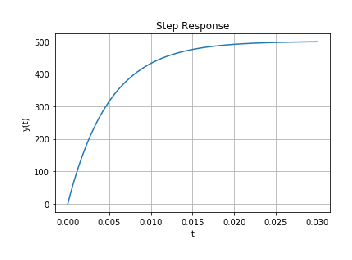
\includegraphics[width=\columnwidth]{./figs/Figure_3.eps}
  \caption{Step Response}
  \label{fig:stepResponse}
\end{figure}
The following code performs all the calculations of above equations
\begin{lstlisting}
codes/code1.py
\end{lstlisting}

The following code plots the open loop gains, closed loop gains and step response to the system
\begin{lstlisting}
codes/code2.py
\end{lstlisting}


\item Designing the circuit for transfer function $T(s)$
\begin{figure}[!hbt]
	\begin{center}
			\resizebox{\columnwidth}{!}{\begin{circuitikz}
\ctikzset{bipoles/length=1cm}
\draw
(0, 0) node[op amp] (opamp) {}
(opamp.-) to[R,l_=$R_1$,-o] (-2, 0.35) -- (-3, 0.35) {}
(opamp.-) to[short,*-] ++(0,0.5) coordinate (leftC)
to[R=$R_2$] (leftC -| opamp.out)
to[short,-*] (opamp.out) to [short,-o] (1.5,0) to (1.5,-0.5) node[ground]{}
(opamp.+) -- (-1,-0.35) to (-1,-0.5) node[ground]{}
(opamp.-) to[short,*-] ++(0,1.5) coordinate (leftC)
to[C=$C_1$] (leftC -| opamp.out) to[short,-*] (opamp.out)

node at (-2.5,0.6){$V_{in}$}
node at (0.75,-0.6){$V_{out}$}
node at (-1.1,1.8){$V_{1}$}
;\end{circuitikz}}
	\end{center}
\caption{Open Loop design}
\label{fig:equivalent_system1}
\end{figure}

1) Designing $G(s)$

Let us assume Op-Amp to be ideal. So this means $V_{1}=0$
Applying KCL at node $V_{1}$

\begin{align}
I_{in} &= I_{C_{1}} + I_{R_{2}}
\\
\dfrac{V_{in}}{R_{1}} &= \dfrac{V_{o1}}{R_{2}} + C_{1}\dfrac{dV_{out}}{dt}
\end{align}
In Laplace domain
\begin{align}
\dfrac{V_{in}(s)}{R_{1}} &= \dfrac{V_{o1}(s)}{R_{2}} + C_{1}sV_{out}(s)
\\
\dfrac{V_{o1}}{V_{in}} &= \dfrac{R_{2}/R_{1}}{1+sR_{2}C_{1}}
\\
\dfrac{V_{o1}}{V_{in}} &= \dfrac{10^{5}}{1+\frac{s}{100}}
\\
\frac{R_{2}}{R_{1}} &= 10^{5}
\\
R_{2}C_{1} &= \frac{1}{100}
\end{align}

As shown in \ref{fig:equivalent_system1} for the two identical poles at 10000 rad/sec we place similar op amp circuits twice.

Solving the circuit for second pole

\begin{align}
\dfrac{V_{o1}(s)}{R_{3}} &= \dfrac{V_{o2}(s)}{R_{4}} + C_{2}sV_{out}(s)
\\
\dfrac{V_{o2}}{V_{o1}} &= \dfrac{R_{4}/R_{3}}{1+sR_{4}C_{2}}
\end{align}

\begin{align}
\dfrac{V_{o2}}{V_{o1}} &= \dfrac{1}{1+\frac{s}{10000}}
\\
\frac{R_{4}}{R_{3}} &= 1
\\
R_{4}C_{2} &= \frac{1}{10000}
\end{align}



2) Designing $H(s) = H$

\begin{figure}[!hbt]
	\begin{center}
			\resizebox{\columnwidth}{!}{\begin{circuitikz}[american]
\draw (0,0)--(-3,0)to [voltage source,l_=$V_i$]++(0,-2)to node[ground]{}++(0,-0.5) ++(6,0)
(0.75,0) node[npn](npn1){Q1}
(npn1.C)--++(0,1.5) to [R,l_=$R_{C1}$]++(0,1.5) to node[ground,rotate=180]{}++(0,0.25)
(npn1.E)-- ++(0,-2) to [R,l_=$R_{E1}$]++(0,-1.5)to node[ground]{}++(0,-0.25)
(npn1.E)++(0,-1)to [R,l_=$R_F$]++(3,0)to[R,l_=$R_{E2}$]++(0,-1.5)to node[ground]{} ++(0,-0.25)
 (4.75,1.5)node[npn](npn2){Q2}
(npn1.C)++(0,0.75)--(npn2.B)
(npn2.E)to node[ground]{}++(0,0)
(npn2.C)--++(0,1.5)to[R,l_=$R_{C2}$]++(0,1.5)to node[ground,rotate=180]{}++(0,0.5)
(8.75,3) node[npn](npn3){Q3}
(npn2.C)++(0,0.75)--(npn3.B)
(npn3.C)to[R,l_=$R_{C3}$]++(0,1.5)to node[ground,rotate=180]{}++(0,0.25)
(npn3.E)to[short,i_=$I_o$]++(0,-2)coordinate(a)to[R,l_=$R_{E2}$]++(0,-1.5)to node[ground]{}++(0,-0.25)
(a)++(0,0.25)to[R,l_=$R_F$]++(3,0)to[R,l_=$R_{E1}$]++(0,-1.5)to node[ground]{}++(0,-0.25);
\draw (-2,-2) node[label={right:$R_i$}]{}--++(0,1.75)--++(0.5,0)[->];
\draw (npn3.E)++(2,-0.5)node[label={right:$R_o$}]{}--++(-1.5,0)[->];


;\end{circuitikz}
}
	\end{center}
\caption{Loop Gain}
\label{fig:equivalent_system4}
\end{figure}

\begin{align}
	V_{out} &= V_{in} \brak{\frac{R_{6}}{R_{5}+R_{6}}}
	\\
	{\frac{R_{6}}{R_{5}+R_{6}}} &= 0.002
	\\
	R_{6} &= 0.002 R_{5}
\end{align}

3) Closed loop design

\begin{figure}[!hbt]
	\begin{center}
			\resizebox{\columnwidth}{!}{\tikzstyle{sum} = [draw, fill=blue!20, circle, node distance=1cm]
\begin{circuitikz}
\ctikzset{bipoles/length=1cm}
\draw
(0, 0) node[op amp] (opamp) {}
(opamp.-) to[R,l_=$R_1$,-o] (-2, 0.35) -- (-3, 0.35) {}
(opamp.-) to[short,*-] ++(0,0.5) coordinate (leftC)
to[R=$R_2$] (leftC -| opamp.out)
to[short,-*] (opamp.out) to [short,-o] (1.5,0) to (1.5,-0.5) node[ground]{}
(opamp.+) -- (-1,-0.35) to (-1,-0.5) node[ground]{}
(opamp.-) to[short,*-] ++(0,1.5) coordinate (leftC)
to[C=$C_1$] (leftC -| opamp.out) to[short,-*] (opamp.out)

node at (-3.3,0.6){$V_{in}$}
node at (1.25,0.4){$V_{out}$}
node at (-1.1,1.8){$V_{1}$}
node at (-2.2,0.1){$-$}
node at (-2.8,0.65){$+$};
\draw (0.75,0) to [short,-o] (0.75,-2) to [R = $R_{3}$, o-] (-1,-2) to [R = $R_{4}$, o-] (-4,-2) to  (-4,-2.5) node[ground]{};
\draw (-1.5,-2) to (-1.5,-1) [short,-o] to (-2.5,-1) [short,-o]  to (-2.5,0.35) node[sum]{};

\end{circuitikz}
}
	\end{center}
\caption{Closed Loop Circuit}
\label{closedloop}
\end{figure}

Figure \ref{closedloop} is the final closed loop design for transfer function $T(s)$

\begin{table}[!ht]
\centering

%%%%%%%%%%%%%%%%%%%%%%%%%%%%%%%%%%%%%%%%%%%%%%%%%%%%%%%%%%%%%%%%%%%%%%
%%                                                                  %%
%%  This is the header of a LaTeX2e file exported from Gnumeric.    %%
%%                                                                  %%
%%  This file can be compiled as it stands or included in another   %%
%%  LaTeX document. The table is based on the longtable package so  %%
%%  the longtable options (headers, footers...) can be set in the   %%
%%  preamble section below (see PRAMBLE).                           %%
%%                                                                  %%
%%  To include the file in another, the following two lines must be %%
%%  in the including file:                                          %%
%%        \def\inputGnumericTable{}                                 %%
%%  at the beginning of the file and:                               %%
%%        \input{name-of-this-file.tex}                             %%
%%  where the table is to be placed. Note also that the including   %%
%%  file must use the following packages for the table to be        %%
%%  rendered correctly:                                             %%
%%    \usepackage[latin1]{inputenc}                                 %%
%%    \usepackage{color}                                            %%
%%    \usepackage{array}                                            %%
%%    \usepackage{longtable}                                        %%
%%    \usepackage{calc}                                             %%
%%    \usepackage{multirow}                                         %%
%%    \usepackage{hhline}                                           %%
%%    \usepackage{ifthen}                                           %%
%%  optionally (for landscape tables embedded in another document): %%
%%    \usepackage{lscape}                                           %%
%%                                                                  %%
%%%%%%%%%%%%%%%%%%%%%%%%%%%%%%%%%%%%%%%%%%%%%%%%%%%%%%%%%%%%%%%%%%%%%%



%%  This section checks if we are begin input into another file or  %%
%%  the file will be compiled alone. First use a macro taken from   %%
%%  the TeXbook ex 7.7 (suggestion of Han-Wen Nienhuys).            %%
\def\ifundefined#1{\expandafter\ifx\csname#1\endcsname\relax}


%%  Check for the \def token for inputed files. If it is not        %%
%%  defined, the file will be processed as a standalone and the     %%
%%  preamble will be used.                                          %%
\ifundefined{inputGnumericTable}

%%  We must be able to close or not the document at the end.        %%
	\def\gnumericTableEnd{\end{document}}


%%%%%%%%%%%%%%%%%%%%%%%%%%%%%%%%%%%%%%%%%%%%%%%%%%%%%%%%%%%%%%%%%%%%%%
%%                                                                  %%
%%  This is the PREAMBLE. Change these values to get the right      %%
%%  paper size and other niceties.                                  %%
%%                                                                  %%
%%%%%%%%%%%%%%%%%%%%%%%%%%%%%%%%%%%%%%%%%%%%%%%%%%%%%%%%%%%%%%%%%%%%%%

	\documentclass[12pt%
			  %,landscape%
                    ]{report}
       \usepackage[latin1]{inputenc}
       \usepackage{fullpage}
       \usepackage{color}
       \usepackage{array}
       \usepackage{longtable}
       \usepackage{calc}
       \usepackage{multirow}
       \usepackage{hhline}
       \usepackage{ifthen}



%%  End of the preamble for the standalone. The next section is for %%
%%  documents which are included into other LaTeX2e files.          %%
\else

%%  We are not a stand alone document. For a regular table, we will %%
%%  have no preamble and only define the closing to mean nothing.   %%
    \def\gnumericTableEnd{}

%%  If we want landscape mode in an embedded document, comment out  %%
%%  the line above and uncomment the two below. The table will      %%
%%  begin on a new page and run in landscape mode.                  %%
%       \def\gnumericTableEnd{\end{landscape}}
%       \begin{landscape}


%%  End of the else clause for this file being \input.              %%
\fi

%%%%%%%%%%%%%%%%%%%%%%%%%%%%%%%%%%%%%%%%%%%%%%%%%%%%%%%%%%%%%%%%%%%%%%
%%                                                                  %%
%%  The rest is the gnumeric table, except for the closing          %%
%%  statement. Changes below will alter the table's appearance.     %%
%%                                                                  %%
%%%%%%%%%%%%%%%%%%%%%%%%%%%%%%%%%%%%%%%%%%%%%%%%%%%%%%%%%%%%%%%%%%%%%%

\providecommand{\gnumericmathit}[1]{#1} 
%%  Uncomment the next line if you would like your numbers to be in %%
%%  italics if they are italizised in the gnumeric table.           %%
%\renewcommand{\gnumericmathit}[1]{\mathit{#1}}
\providecommand{\gnumericPB}[1]%
{\let\gnumericTemp=\\#1\let\\=\gnumericTemp\hspace{0pt}}
 \ifundefined{gnumericTableWidthDefined}
        \newlength{\gnumericTableWidth}
        \newlength{\gnumericTableWidthComplete}
        \newlength{\gnumericMultiRowLength}
        \global\def\gnumericTableWidthDefined{}
 \fi
%% The following setting protects this code from babel shorthands.  %%
 \ifthenelse{\isundefined{\languageshorthands}}{}{\languageshorthands{english}}
%%  The default table format retains the relative column widths of  %%
%%  gnumeric. They can easily be changed to c, r or l. In that case %%
%%  you may want to comment out the next line and uncomment the one %%
%%  thereafter                                                      %%
\providecommand\gnumbox{\makebox[0pt]}
%%\providecommand\gnumbox[1][]{\makebox}

%% to adjust positions in multirow situations                       %%
\setlength{\bigstrutjot}{\jot}
\setlength{\extrarowheight}{\doublerulesep}

%%  The \setlongtables command keeps column widths the same across  %%
%%  pages. Simply comment out next line for varying column widths.  %%
\setlongtables

\setlength\gnumericTableWidth{%
	53pt+%
	93pt+%
0pt}
\def\gumericNumCols{2}
\setlength\gnumericTableWidthComplete{\gnumericTableWidth+%
         \tabcolsep*\gumericNumCols*2+\arrayrulewidth*\gumericNumCols}
\ifthenelse{\lengthtest{\gnumericTableWidthComplete > \linewidth}}%
         {\def\gnumericScale{\ratio{\linewidth-%
                        \tabcolsep*\gumericNumCols*2-%
                        \arrayrulewidth*\gumericNumCols}%
{\gnumericTableWidth}}}%
{\def\gnumericScale{1}}

%%%%%%%%%%%%%%%%%%%%%%%%%%%%%%%%%%%%%%%%%%%%%%%%%%%%%%%%%%%%%%%%%%%%%%
%%                                                                  %%
%% The following are the widths of the various columns. We are      %%
%% defining them here because then they are easier to change.       %%
%% Depending on the cell formats we may use them more than once.    %%
%%                                                                  %%
%%%%%%%%%%%%%%%%%%%%%%%%%%%%%%%%%%%%%%%%%%%%%%%%%%%%%%%%%%%%%%%%%%%%%%

\ifthenelse{\isundefined{\gnumericColA}}{\newlength{\gnumericColA}}{}\settowidth{\gnumericColA}{\begin{tabular}{@{}p{60pt*\gnumericScale}@{}}x\end{tabular}}
\ifthenelse{\isundefined{\gnumericColB}}{\newlength{\gnumericColB}}{}\settowidth{\gnumericColB}{\begin{tabular}{@{}p{60pt*\gnumericScale}@{}}x\end{tabular}}

\begin{tabular}[c]{%
	b{\gnumericColA}%
	b{\gnumericColB}%
	}

%%%%%%%%%%%%%%%%%%%%%%%%%%%%%%%%%%%%%%%%%%%%%%%%%%%%%%%%%%%%%%%%%%%%%%
%%  The longtable options. (Caption, headers... see Goosens, p.124) %%
%	\caption{The Table Caption.}             \\	%
% \hline	% Across the top of the table.
%%  The rest of these options are table rows which are placed on    %%
%%  the first, last or every page. Use \multicolumn if you want.    %%

%%  Header for the first page.                                      %%
%	\multicolumn{2}{c}{The First Header} \\ \hline 
%	\multicolumn{1}{c}{colTag}	%Column 1
%	&\multicolumn{1}{c}{colTag}	\\ \hline %Last column
%	\endfirsthead

%%  The running header definition.                                  %%
%	\hline
%	\multicolumn{2}{l}{\ldots\small\slshape continued} \\ \hline
%	\multicolumn{1}{c}{colTag}	%Column 1
%	&\multicolumn{1}{c}{colTag}	\\ \hline %Last column
%	\endhead

%%  The running footer definition.                                  %%
%	\hline
%	\multicolumn{2}{r}{\small\slshape continued\ldots} \\
%	\endfoot

%%  The ending footer definition.                                   %%
%	\multicolumn{2}{c}{That's all folks} \\ \hline 
%	\endlastfoot
%%%%%%%%%%%%%%%%%%%%%%%%%%%%%%%%%%%%%%%%%%%%%%%%%%%%%%%%%%%%%%%%%%%%%%

\hhline{|-|-}
	 \multicolumn{1}{|p{\gnumericColA}|}%
	{\gnumericPB{\centering}\gnumbox{\textbf{Parameter}}}
	&\multicolumn{1}{p{\gnumericColB}|}%
	{\gnumericPB{\centering}\gnumbox{\textbf{Value}}}
\\
\hhline{|-|-}
	 \multicolumn{1}{|p{\gnumericColA}|}%
	{\gnumericPB{\centering}\gnumbox{\text{$R$}}}
	&\multicolumn{1}{p{\gnumericColB}|}%
	{\gnumericPB{\centering}\gnumbox{\text{$1000\Omega$}}}
\\
\hhline{|-|-}
	 \multicolumn{1}{|p{\gnumericColA}|}%
	{\gnumericPB{\centering}\gnumbox{\text{$R_f$}}}
	&\multicolumn{1}{p{\gnumericColB}|}%
	{\gnumericPB{\centering}\gnumbox{\text{$2000\Omega$}}}
\\
\hhline{|-|-}
	 \multicolumn{1}{|p{\gnumericColA}|}%
	{\gnumericPB{\centering}\gnumbox{\text{$C$}}}
	&\multicolumn{1}{p{\gnumericColB}|}%
	{\gnumericPB{\centering}\gnumbox{\text{$7.9577\times10^{-10}$}}}
\\
\hhline{|-|-|}
\end{tabular}

\ifthenelse{\isundefined{\languageshorthands}}{}{\languageshorthands{\languagename}}
\gnumericTableEnd

\caption{Circuit Parameters}
\label{table:DesignParams}
\end{table}

The table \ref{table:DesignParams} provides the parameters for our circuit design. 

The arbitrary parameters can be selected based on practical availability.


\item Verification of closed loop circuit design through SPICE


\begin{figure}[!ht]
\centering
    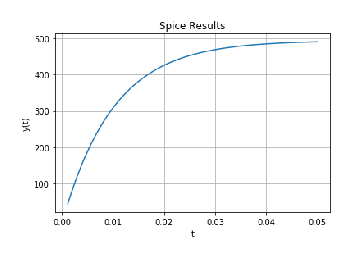
\includegraphics[width=\columnwidth]{./figs/Figure_4.eps}
  \caption{SPICE simulation of circuit \ref{fig:equivalent_system1}}
  \label{fig:SPICEresult}
\end{figure}

A SPICE simulation of circuit \ref{fig:equivalent_system1} is done by providing a DC input(Unit Step Input). 

The obtained plot (figure \ref{fig:SPICEresult}) is similar to the Step response of the feedback system in figure \ref{fig:stepResponse}. Hence we verify our design is correct.


The following code plots the SPICE simulation results
from SPICE plot .dat file and spice .net file

\begin{lstlisting}
codes/spice/plotter.py
\end{lstlisting}

The following is the spice simulation file

\begin{lstlisting}
codes/spice/spice.net
\end{lstlisting}

For instructions to run the spice simulation please refer

\begin{lstlisting}
codes/spice/readme.md
\end{lstlisting}
\end{enumerate}